
\documentclass[12pt]{amsart}
\usepackage{geometry} % see geometry.pdf on how to lay out the page. There's lots.
\usepackage{graphicx} 
\geometry{a4paper} % or letter or a5paper or ... etc
% \geometry{landscape} % rotated page geometry





% See the ``Article customise'' template for come common customisations


\title{}
\author{}
\date{} % delete this line to display the current date


\makeatletter %?\section???????
\renewcommand{\section}{\@startsection{section}{1}{0mm}
  {-\baselineskip}{0.5\baselineskip}{\bf\leftline}}
\makeatother



%%% BEGIN DOCUMENT
\begin{document}
\section{Software Design}

\subsection{\textbf{Implementation Decision}}

\subsubsection{\textbf{Agile software development: Scrum}}
\paragraph{According to Jonathan, it is possible that Scrum is used most commonly nowadays, which is a framework for project management. The purpose of using Scrum is to encourage teams to organize tasks themselves and iteratively deliver functionality in a sprint, which we decide as ten days. Scrum perfectly fits our condition where our stakeholder changes his requirement frequently and asks us to release the fist version of the software in one and a half month. There are two important roles, product owner and scrum master. Product owner Shulan is responsible for contacting with our stakeholder and convey what the software supposed to be. Scrum master Chengfeng is in charge of daily standup meetings and burn down chart. At the beginning of each sprint, we have a sprint planning meeting to decide sprint backlog and estimate time consuming. After each sprint, a retrospective meeting is held for doing better in the next sprint. A general process of Scrum is shown in Figure 1. By using Scrum, there is no need that all requirements should be specified clearly at the beginning. Besides, a lot of documentation jobs are reduced.}

\begin{center}
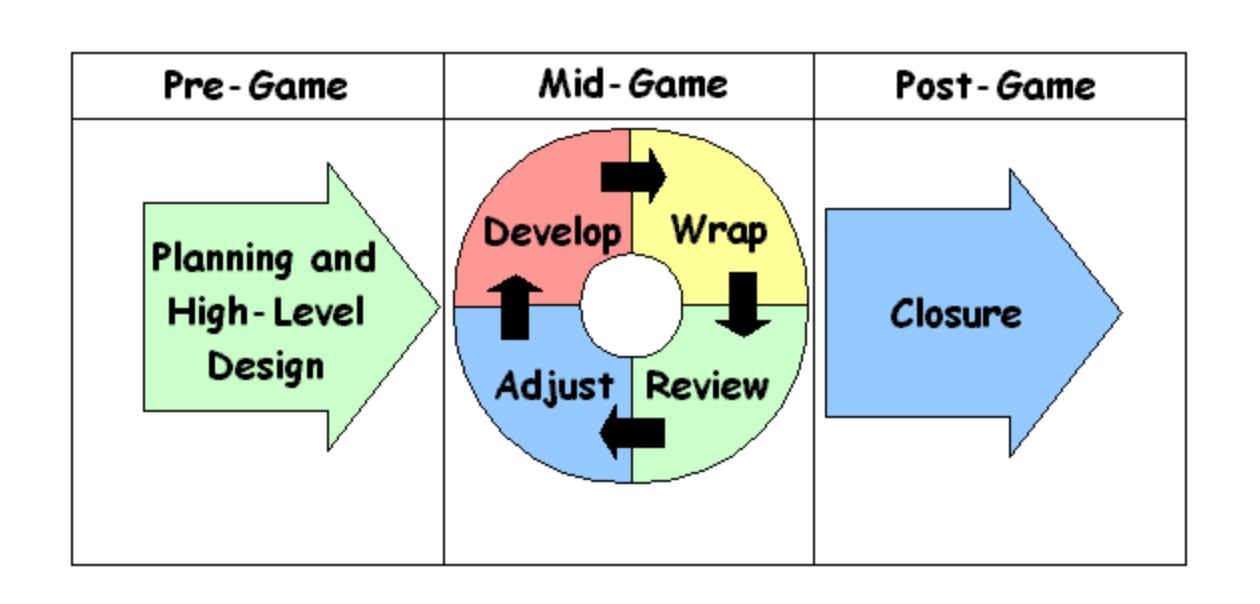
\includegraphics[width=0.8\linewidth]{scrum.png}
\centerline{Figure 1: General Scrum Process (Marc, J. Dunlap, 2003)}
\end{center}


\subsubsection{\textbf{Task assignment platform: Worktile}}
\paragraph{Worktile is the online platform we use to arrange and assign tasks efficiently. It uses board to manage tasks, providing function to browsing and sorting tasks list. We put all our user stories as on task board and assign them to members. There are three boards in every member's interface, to-do task board, in-doing task board and finished task board. Every member arranges his/her tasks to them. By using Worktile, every member can specifically understand the process of his/her jobs and arrange time scientifically. Besides, it is clear to see the state of each task and save a lot of time in task arrangement.}



\subsubsection{\textbf{Peer coding platform: Github}}
\paragraph{
We choose Github to insist our peer coding because it is useful in the two most fundamental aspects version control and code sharing during our programming.  Github is a hosting service to use Git, which is a version control system. With Git, almost every operation is conducted locally, which makes it fast on  centralized systems communicating with another server in somewhere else. Besides, Git written by C language, which is able to reduce overhead runtimes causing by higher-level languages.
The way Git uses to distribute is that the user have a "clone" of the whole repository. This means each user essentially having a complete backup of main server. Every copy is able to replace the main server in the condition that a corruption or crash occurs. So, it is convenient for our group project. As the initial version of code is pushed to our public repository, each member can contribute to editing code and others can see it immediately. If there exists a problem in the edited code, we can back to use the previous one. By using Github, it is time-saving to share code in the group and making it clear in version control of our project.}


\subsubsection{\textbf{Reference}}
\paragraph{http://www.agilenutshell.com/scrum}
\paragraph{https://www.atlassian.com/agile/scrum}
\paragraph{https://git-scm.com}

\end{document}